%%%%%%%%%%%%%%%%%%%%%%%%%%%%%%%%%%%%%%%%%%%%%%%%%%%%%%%%%%%%%%%%%%%%%%%%%%%%%%%%
%% Copyright (C) 2010 Gleb Belov <bg37@gmx.net>.
%%
%% This file is part of caparf (http://code.google.com/p/caparf/).
%%
%% caparf is free software: you can redistribute it and/or modify
%% it under the terms of the GNU General Public License as published by
%% the Free Software Foundation, either version 3 of the License, or
%% (at your option) any later version.
%%
%% caparf is distributed in the hope that it will be useful,
%% but WITHOUT ANY WARRANTY; without even the implied warranty of
%% MERCHANTABILITY or FITNESS FOR A PARTICULAR PURPOSE. See the
%% GNU General Public License for more details.
%%
%% You should have received a copy of the GNU General Public License
%% along with caparf. If not, see <http://www.gnu.org/licenses/>.
%%%%%%%%%%%%%%%%%%%%%%%%%%%%%%%%%%%%%%%%%%%%%%%%%%%%%%%%%%%%%%%%%%%%%%%%%%%%%%%%

\documentclass[a4paper,12pt]{article}

\addtolength{\topmargin}{-2.3cm}
\addtolength{\textheight}{4.3cm}
\oddsidemargin-1mm
\addtolength{\textwidth}{3.3cm}
\renewcommand{\baselinestretch}{0.95}

\usepackage{color}
\usepackage{hyperref}
\usepackage{wrapfig}
\usepackage{graphicx}
\usepackage{amsmath}
\usepackage{amsthm}
\usepackage{amsfonts}
\usepackage[scaled]{helvet}
\renewcommand*\familydefault{\sfdefault}

\sloppy

\begin{document}

\newcommand{\itemh}[2]{\item[{\makebox[9mm][l]{\bf{#1}}}] \textbf{#2}
\nopagebreak}

\title{Orthogonal packing problems overview}

\section{Inroduction}

Orthogonal packing in two and more dimensions includes a family of problems that are relevant in production and scheduling \cite{ESICUP,WaescherTyp,Hartmann2000}, reconfigurable computing \cite{Wiki-ReconfComp}, transport and warehouse logistics. We consider $d$-dimensional rectangular objects, items (boxes) and container(s) with integer sizes $w^k_i$ and $W_k$, respectively, for $k=\overline{1,d}$ and $i=\overline{1,n}$. The items should be packed into the container(s) with their sides parallel to those of the container, without rotations. 

The basic problem is the \emph{$d$-Dimensional Orthogonal Packing Problem} (OPP). This is a \emph{decision problem} which asks whether all given items fit into the given container. OPP belongs to the class of \emph{strongly $\mathcal{NP}$-complete} problems \cite{GJ79,FekExact}. By defining an objective function and further constraints we can distinguish other types of $d$-dimensional orthogonal packing problems, e.g.,
\begin{enumerate}
\item the \emph{Strip-Packing Problem} (SPP) consists in minimizing the height $W_d$ of a container that can hold all boxes, where the sizes $W_1$, $W_2$, \ldots, $W_{d-1}$ of the other dimensions of the container are fixed;
\item the \emph{Orthogonal Bin-Packing Problem} (BPP) consists in determining the minimal number of identical containers that are required to pack all the items; 
\item the \emph{Orthogonal Knapsack Problem} (OKP) consists in maximizing the total value of a subset of the boxes packable into the given container with the assumption that every box has a certain value.
\end{enumerate}

The problems 1.--3.\ are \emph{optimization problems} because they have an objective function. They are \emph{strongly $\mathcal{NP}$-hard} \cite{GJ79,FekExact}. The corresponding solution methods typically rely on those for OPP, that is why it is important to study this basic decision problem.


\section{Relaxations and bounds}

Many solution methods use \emph{bounds on the solution value}. For example, the simplest bound for OPP is the \emph{volume bound}: if the total volume of the items exceeds that of the container, then the instance is infeasible.   Bounds are obtained from \emph{relaxations} of the main problem, i.e., somewhat simpler problems. Bounds should be preferably quickly computable. However, some bounds are so strong that it pays off to spend more time for their computation. In many methods, the following relaxations of orthogonal packing are used to obtain bounds:

\begin{enumerate}
\item \emph{Conservative scales} (CS) \cite{FekBnd} are modified item sizes such that if a packing exists, it is also feasible with the modified sizes. Thus, the volume bound for the modified instance is valid for the original instance. Often it is stronger, which is heavily used in algorithms. CS can be obtained by combinatorial heuristics called \emph{dual-feasible functions} (DFF) \cite{FekBnd,ClaDFFSurvey} and as dual solutions \cite{BiD-BiLin} of the set-partitioning formulation of the simple 1D relaxation (see below).

\item The \emph{simple one-dimensional relaxation} of 2D SPP: instead of $n$ items sized $w_i\times h_i$, we consider \emph{$n$ types} of items with sizes $w_i\times1$; for each type $i=\overline{1,n}$, $h_i$ copies should be packed. This leads to a special \emph{One-Dimensional Cutting-Stock Problem} (1D CSP) \cite{Wiki-1DCSP,GG61,AlvesCarvalho08}: given stock bars of size $W$ and $n$ item types of size $w_i$ and order demands $h_i$, $i=\overline{1,n}$, minimize the number of bars needed to obtain all the items so that each bar has at most one item of each type.

1D CSP itself is $\mathcal{NP}$-hard, that is why its LP bounds are used. The LP relaxation of the \emph{set-partitioning model} of 1D CSP is very tight \cite{GG61,RST02}. It proved very effective for 2D packing \cite{Letch03,BiD-BiLin,Baldacci07,BKS07,Roh08}.

\item The \emph{Cumulative-Resource Non-Preemptive Scheduling Problem}, cf.\ \cite{ClaConstr} or, equivalently, the \emph{One-Dimensional Contiguous Cutting-Stock Problem} (CCSP), cf.\ \cite{MMV03,SPPExactAlvarez}: in terms of scheduling, we have $n$ jobs and a single resource, job $i$ consumes $w_i$ units of the resource for $h_i$ units of time. Each job should be processed without interruption (\emph{non-preemptiveness}). The resource can be consumed cumulatively, but in any moment of time up to $W$ units. The goal is to minimize the total processing time. This is a relaxation of the two-dimensional SPP: the geometry of the items in one dimension is relaxed, see Figure~\ref{figCCSP}. Thus, any feasible SPP layout is feasible for CCSP. Note that 1D CSP is a relaxation of CCSP.
\begin{figure}[htb]

\qquad
\begin{minipage}{0.9\textwidth}
\centering

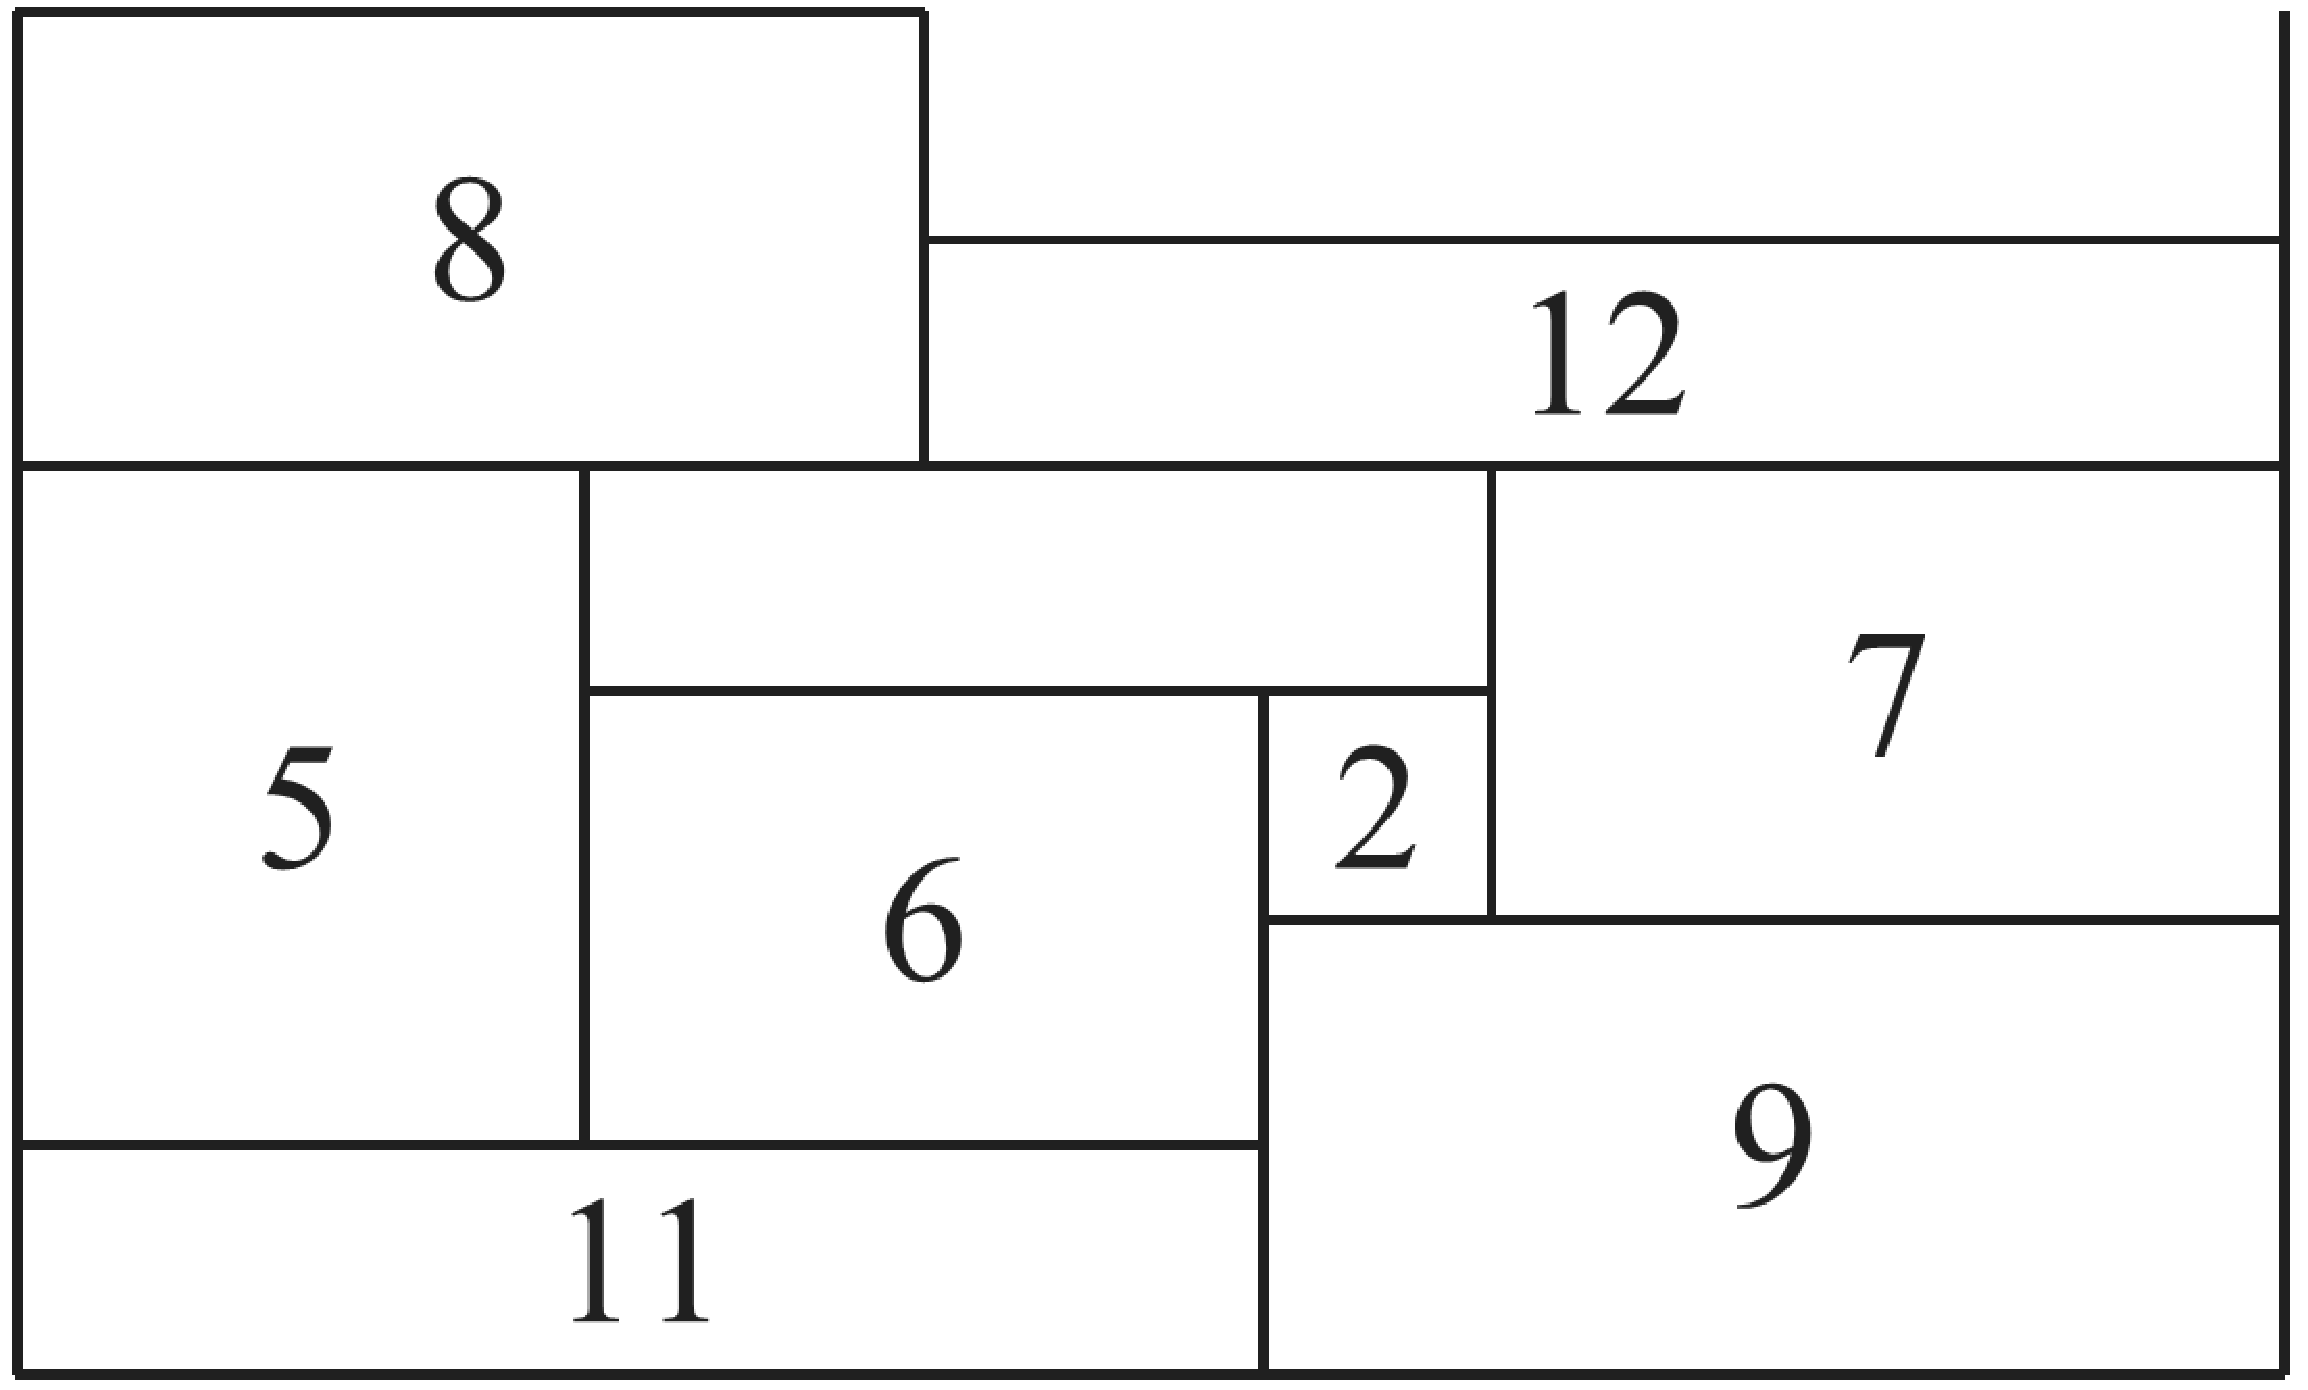
\includegraphics[width=0.4\textwidth]{ctg1_opp}
\hfill
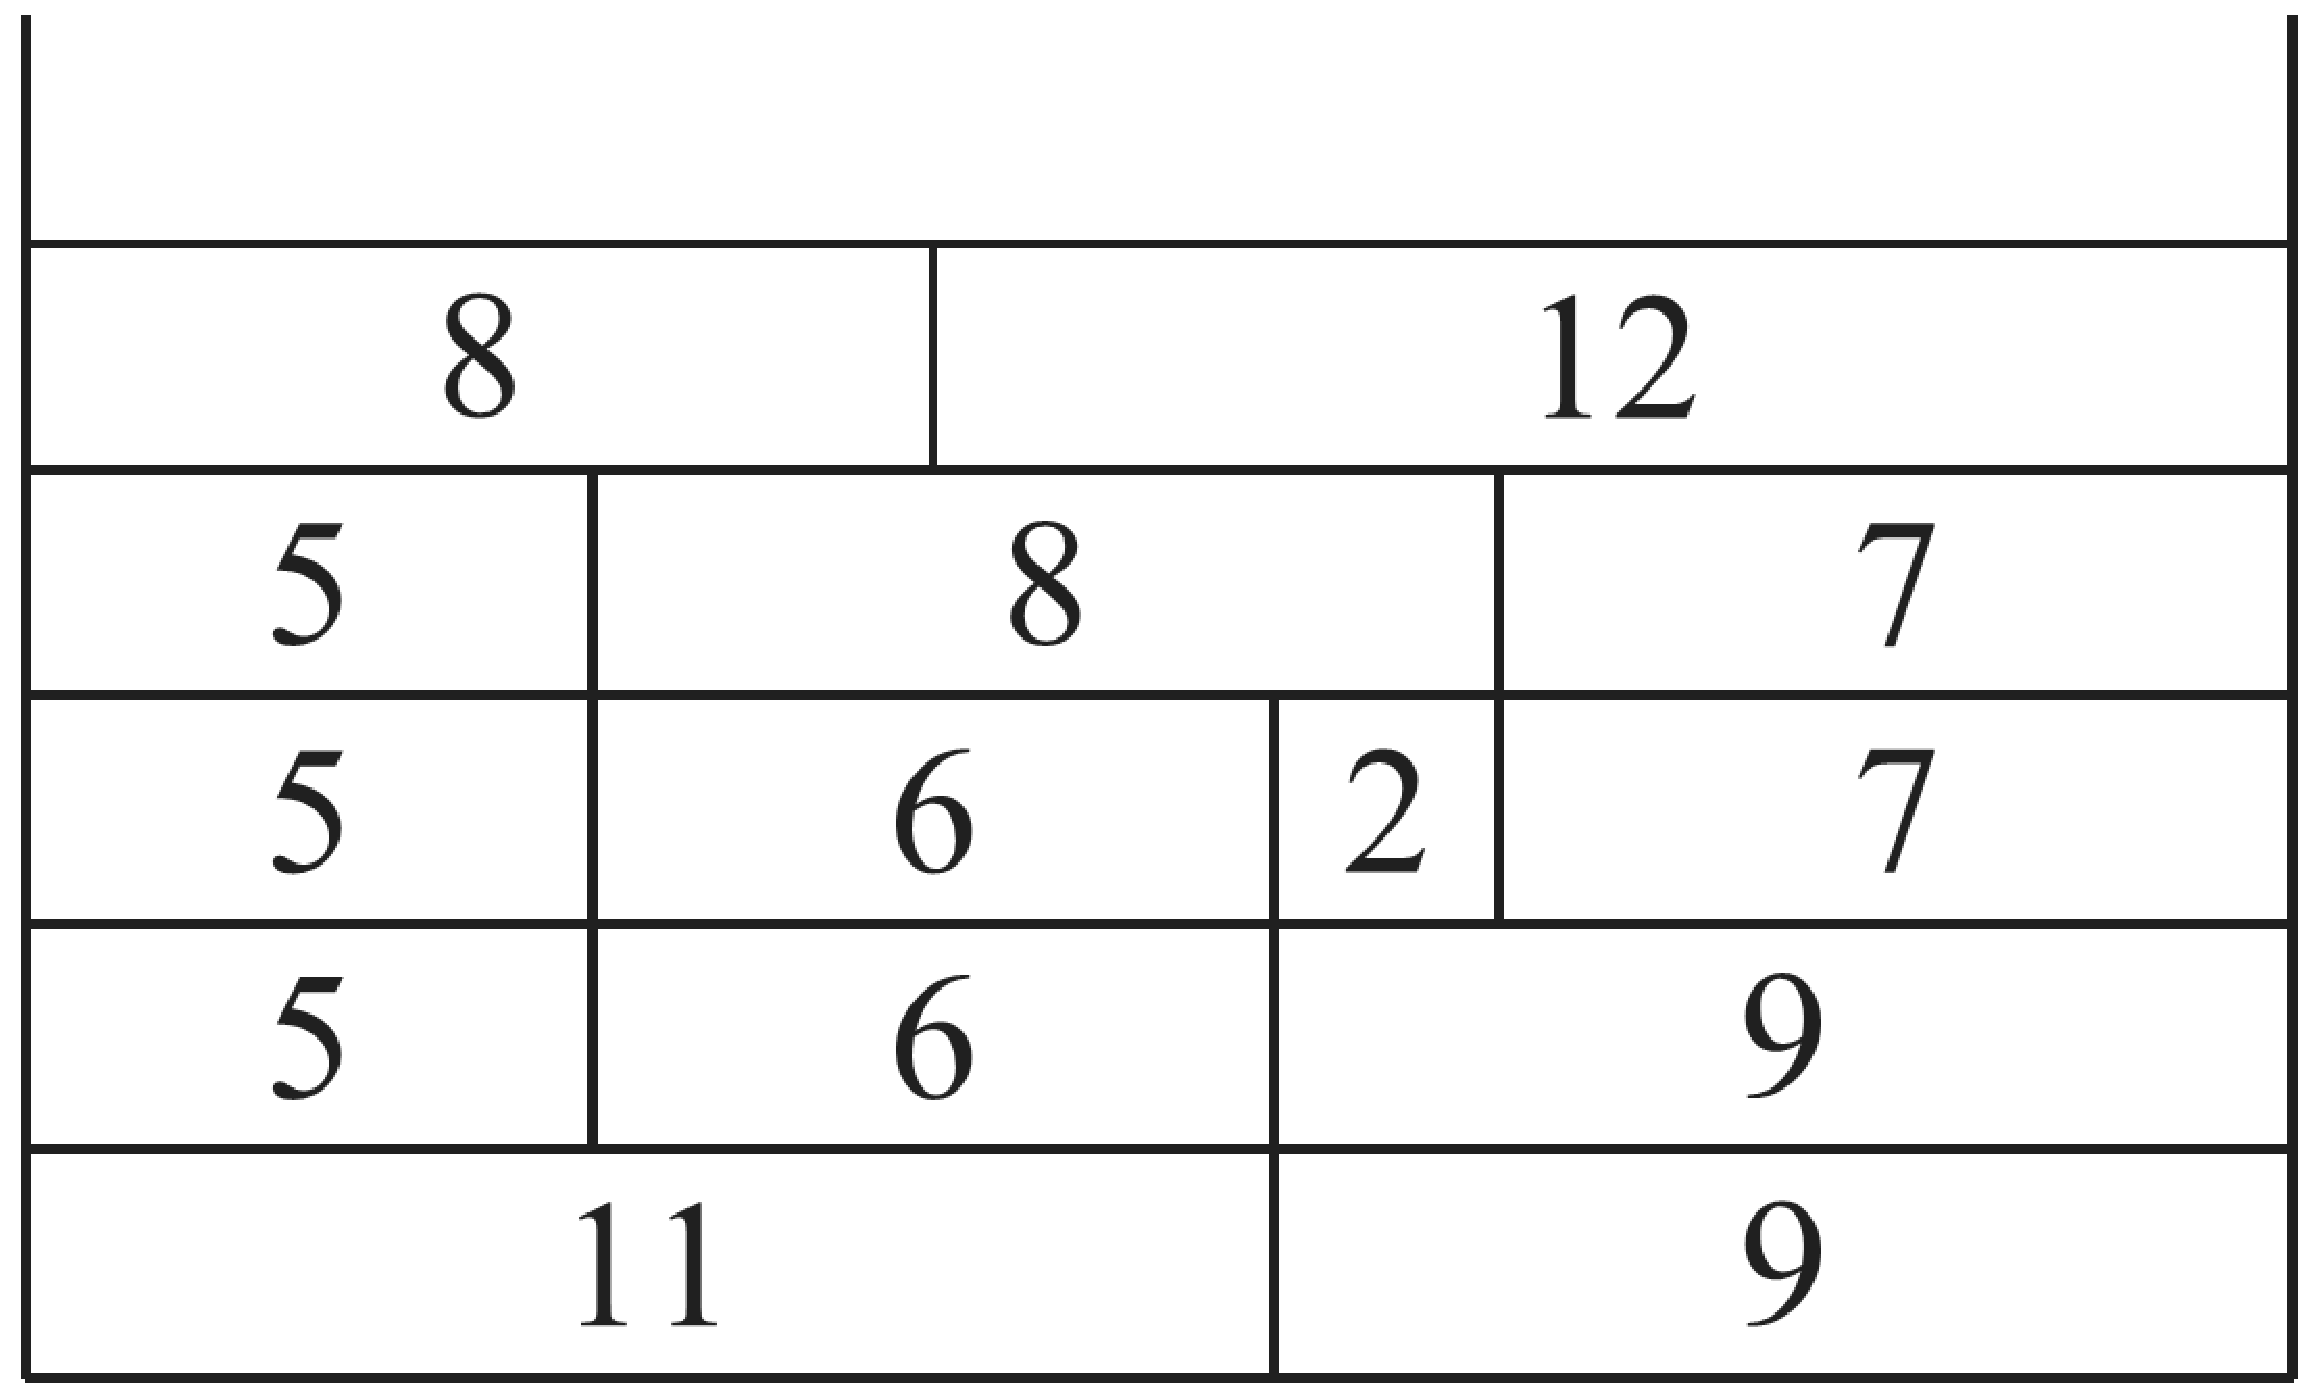
\includegraphics[width=0.4\textwidth]{ctg1}

\caption{\label{figCCSP}An instance of 2D SPP and a corresponding non-preemptive cumulative-resource schedule of CCSP \cite{Sch08}. In this case, the latter coincides with an optimum of the corresponding 1D CSP. The numbers denote item widths $w_i$, $i=\overline{1,n}$.}
\end{minipage}
\end{figure}
\end{enumerate}
Thus, the set-partitioning formulation of 1D CSP provides strong bounds for OPP, in particular it delivers good conservative scales. \emph{The LP relaxations of 1D CSP and of CCSP would be the main instruments in the project.}

Further bounds are obtained, e.g., by preprocessing the combinatorial properties of packings: non-overlapping \cite{ClaConstr}, transitivity of item orderings \cite{PisBPP07}, transitive orientability of the overlapping relations and containment \cite{FekExactLarge} and others.

\section{Models and exact algorithms for OPP and SPP}

Exact methods for strongly $\mathcal{NP}$-hard problems are typically based on \emph{branch-and-bound} which is the most efficient technique for such problems nowadays \cite{NW88}. Branch-and-bound is a principle to separate the solution space and prune unpromising parts using bounds. For the computational success, of crucial importance are both the \emph{branching strategy} and the employed bounds, which typically depend on the chosen \emph{model} of the problem \cite{NW88}.

Thus, to begin our classification of exact methods, we start with the known models of OPP. The ``natural'' OPP model defines item coordinates as variables and just states the containment and non-overlapping conditions:

\emph{Find a set of coordinates $x^k_i$, $k=\overline{1,d}$, $i=\overline{1,n}$, satisfying}
\begin{subequations} \label{modOPP}
\begin{align}
0\le x^k_i \le W_k - w^k_i &  \quad \forall k, i, \label{modOPPcnt} \\
x^k_i + w^k_i \le x^k_j \quad \text{or} \quad x^k_j + w^k_j \le x^k_i &  \quad \text{for at least one $k$, }\quad \forall i < j, \label{modOPPord} %\tag{non-overlapping}
\end{align}
\end{subequations}
\emph{or prove that none exist.}

Today's most successful approaches to OPP are based on this model implemented using Constraint Programming (CP) \cite{ClaConstr,SimonisSearch,BeldiceanuCP08,PisBPP07}. The method in \cite{ClaConstr} uses branching and bounding techniques from scheduling problems. 

Another powerful model is the graph-theoretical model of Fekete and Schepers \cite{FekExact}. It considers the intersection relations of the item projections on each axis, which are described by the so-called \emph{intersection graphs}. Given a system of $d$ such graphs (one for each dimension), called \emph{packing class}, we can restore the item orderings along each axis and, finally, the coordinates. Thus, the goal of a corresponding enumeration scheme is to obtain a packing class. Note that item orderings and coordinates are handled implicitly. Branching is performed on the edges of the graphs. The bounds use, e.g., the combinatorial properties of the graphs (intervalness). The corresponding exact algorithm \cite{FekExactLarge} proved very efficient both for OPP as well as for OKP in two and three dimensions. Belov and Rohling \cite{BR09} improved this algorithm by introducing bounds and branching strategy based on the 1D cutting-stock LP relaxation. However, this algorithm is not as strong as that based on CP \cite{ClaConstr}.

Other methods are much less efficient. They use, e.g., the direct layout coding \cite{MMV03,SPPExactAlvarez} or Integer Linear Programming (ILP) formulations \cite{Pad00,Baldacci07}.

\section{Today's exact algorithms for OKP and BPP}

For the 2D knapsack problem, one of the latest algorithms is \cite{Baldacci07}. It has a two-level enumeration scheme: at the first level, all candidate subsets of items that could fit into the knapsack are enumerated. For each such subset, the corresponding OPP is solved as an ILP by commercial software. At the first level, strong LP bounds based on 1D CSP are applied, which lead to very strong decrease of the number of candidate subsets. The branching strategy in the first level is \emph{LP-based}, i.e., the solutions of the LP give hints for branching variable selection.

For bin packing, the exact algorithm in \cite{PisBPP07} uses LP in the upper level (to combine whole bins), and Constraint Programming to pack the bins by solving OKPs. The algorithm can be seen as a merge of CP and LP techniques. Another exact method \cite{ClaBPPExact} is purely combinatorial.

\section{Today's heuristic algorithms}\nopagebreak

Heuristics are non-exact algorithms mostly based on \emph{intuitive principles} aimed at quickly finding good solutions. They allow the efficient handling of complicated constraints, e.g., industrial ones.
For orthogonal packing, all published heuristics are, to the best of our knowledge, purely combinatorial. For literature reviews, see, e.g., \cite{Egeblad09,BSM-SVC2,GRASPbpp}.

\begin{thebibliography}{10}

\bibitem[AV08]{AlvesCarvalho08}
C.~Alves and J.~M. {Val\'erio de Carvalho}.
\newblock A stabilized branch-and-price-and-cut algorithm for the multiple
  length cutting stock problem.
\newblock {\em Computers \& Operations Research}, 35(4):1315--1328, 2008.

\bibitem[AVPT09]{SPPExactAlvarez}
R.~Alvarez-Valdes, F.~Parre{\~n}o, and J.~M. Tamarit.
\newblock A branch and bound algorithm for the strip packing problem.
\newblock {\em OR Spectrum}, 31(2):431--459, 2009.

\bibitem[BB07]{Baldacci07}
R.~Baldacci and M.~A. Boschetti.
\newblock A cutting-plane approach for the two-dimensional orthogonal
  non-guillotine cutting problem.
\newblock {\em European Journal of Operational Research}, 183(3):1136--1149,
  2007.

\bibitem[BCP08]{BeldiceanuCP08}
N.~Beldiceanu, M.~Carlsson, and E.~Poder.
\newblock New filtering for the \emph{cumulative} constraint in the context of
  non-overlapping rectangles.
\newblock In L.~Perron and M.A. Trick, editors, {\em CPAIOR}, volume 5015 of
  {\em LNCS}, pages 21--35. Springer, 2008.

\bibitem[BKRS09]{BKS07}
G.~Belov, V.~Kartak, H.~Rohling, and G.~Scheithauer.
\newblock One-dimensional relaxations and {LP} bounds for orthogonal packing.
\newblock {\em International Transactions on Operational Research},
  16(6):745--766, 2009.

\bibitem[BR09]{BR09}
G.~Belov and H.~Rohling.
\newblock A branch-and-price graph-theoretical algorithm for orthogonal-packing
  feasibility.
\newblock Preprint MATH-NM-10-2009, Dresden University of Technology, November
  2009.
\newblock Submitted.

\bibitem[BSM08]{BSM-SVC2}
G.~Belov, G.~Scheithauer, and E.~A. Mukhacheva.
\newblock One-dimensional heuristics adapted for two-dimensional rectangular
  strip packing.
\newblock {\em Journal of the Operational Research Society}, 59(6):823--832,
  2008.

\bibitem[CAdC08]{ClaDFFSurvey}
F.~Clautiaux, C.~Alves, and J.~Val{\'e}rio de~Carvalho.
\newblock A survey of dual-feasible functions for bin-packing problems.
\newblock {\em Annals of Operations Research}, 2008.

\bibitem[CCM07]{ClaBPPExact}
F.~Clautiaux, J.~Carlier, and A.~Moukrim.
\newblock A new exact method for the two-dimensional bin-packing problem with
  fixed orientation.
\newblock {\em Operations Research Letters}, 35(3):357 -- 364, 2007.

\bibitem[CJCM08]{ClaConstr}
F.~Clautiaux, A.~Jouglet, J.~Carlier, and A.~Moukrim.
\newblock A new constraint programming approach for the orthogonal packing
  problem.
\newblock {\em Computers {\&} Operations Research}, 35(3):944--959, 2008.

\bibitem[CLM05]{BiD-BiLin}
A.~Caprara, M.~Locatelli, and M.~Monaci.
\newblock Bidimensional packing by bilinear programming.
\newblock In M.~{J\"unger} and V.~Kaibel, editors, {\em Proceedings of the
  Eleventh Conference on Integer Programming and Combinatorial Optimization
  (IPCO'05)}, LNCS 3509, pages 377--391. Springer-Verlag, 2005.

\bibitem[EP09]{Egeblad09}
J.~Egeblad and D.~Pisinger.
\newblock Heuristic approaches for the two- and three-dimensional knapsack
  packing problem.
\newblock {\em Computers \& Operations Research}, 36(4):1026 -- 1049, 2009.

\bibitem[ESI]{ESICUP}
{EURO} special interest group on cutting and packing ({ESICUP}).
\newblock \emph{http://paginas.fe.up.pt/\~{ }esicup/}, accessed 25 November
  2008.

\bibitem[FS04a]{FekExact}
S.~P. Fekete and J.~Schepers.
\newblock A combinatorial characterization of higher-dimensional orthogonal
  packing.
\newblock {\em Mathematics of Operations Research}, 29(2):353--368, 2004.

\bibitem[FS04b]{FekBnd}
S.~P. Fekete and J.~Schepers.
\newblock A general framework for bounds for higher-dimensional orthogonal
  packing problems.
\newblock {\em Mathematical Methods of Operations Research}, 60(2):311--329,
  2004.

\bibitem[FSvdV07]{FekExactLarge}
S.~P. Fekete, J.~Schepers, and J.~van~der Veen.
\newblock An exact algorithm for higher-dimensional orthogonal packing.
\newblock {\em Operations Research}, 55(3):569--587, 2007.

\bibitem[GG61]{GG61}
P.~C. Gilmore and R.~E. Gomory.
\newblock A linear programming approach to the cutting-stock problem ({P}art
  {I}).
\newblock {\em Oper. Res.}, 9:849--859, 1961.

\bibitem[GJ79]{GJ79}
M.~R. Garey and D.~S. Johnson.
\newblock {\em Computers and intractability}.
\newblock Freeman, 1979.

\bibitem[Har00]{Hartmann2000}
S.~Hartmann.
\newblock {\em Project Scheduling Under Limited Resources}.
\newblock Springer, 2000.

\bibitem[LA01]{Letch03}
A.~N. Letchford and A.~Amaral.
\newblock Analysis of upper bounds for the pallet loading problem.
\newblock {\em European Journal of Operational Research}, 132(3):582--593,
  2001.

\bibitem[MMV03]{MMV03}
S.~Martello, M.~Monaci, and D.~Vigo.
\newblock An exact approach to the strip-packing problem.
\newblock {\em INFORMS Journal on Computing}, 15(3):310--319, 2003.

\bibitem[NW88]{NW88}
G.~L. Nemhauser and L.~A. Wolsey.
\newblock {\em Integer and Combinatorial Optimization}.
\newblock John Wiley and Sons, New York, 1988.

\bibitem[Pad00]{Pad00}
M.~Padberg.
\newblock Packing small boxes into a big box.
\newblock {\em Mathematical Methods of Operations Research}, 52(1):1--21, 2000.

\bibitem[PAVOT08]{GRASPbpp}
F.~Parre{\~n}o, R.~Alvarez-Valdes, J.~F. Oliveira, and J.~M. Tamarit.
\newblock A hybrid {GRASP/VND} algorithm for two- and three-dimensional bin
  packing.
\newblock {\em Annals of Operations Research}, 2008.

\bibitem[PS07]{PisBPP07}
D.~Pisinger and M.~M. Sigurd.
\newblock Using decomposition techniques and constraint programming for solving
  the two-dimensional bin-packing problem.
\newblock {\em INFORMS Journal on Computing}, 19(1):36--51, 2007.

\bibitem[Roh08]{Roh08}
H.~Rohling.
\newblock {\em {LP} bounds in exact algorithms for two-dimensional orthogonal
  packing}.
\newblock Diploma thesis, Dresden University, November 2008.
\newblock In German.

\bibitem[RST02]{RST02}
J.~Rietz, G.~Scheithauer, and J.~Terno.
\newblock Families of non-{IRUP} instances of the one-dimensional cutting stock
  problem.
\newblock {\em Discrete Applied Mathematics}, 121:229--245, 2002.

\bibitem[Sch08]{Sch08}
G.~Scheithauer.
\newblock {\em Cutting and Packing Problems}.
\newblock Vieweg+Teubner Verlag, 2008.
\newblock In German.

\bibitem[SO08]{SimonisSearch}
H.~Simonis and B.~O'Sullivan.
\newblock Search strategies for rectangle packing.
\newblock In P.J. Stuckey, editor, {\em Principles and Practice of Constraint
  Programming}, volume 5202 of {\em LNCS}, pages 52--66. Springer, 2008.

\bibitem[WHS07]{WaescherTyp}
G.~Wascher, H.~Hau{\ss}ner, and H.~Schumann.
\newblock An improved typology of cutting and packing problems.
\newblock {\em European Journal of Operational Research}, 183(3):1109--1130,
  2007.

\bibitem[{Wik}08]{Wiki-1DCSP}
{Wikipedia contributors}.
\newblock Cutting stock problem, eindimensionales {Z}uschnittproblem.
\newblock {\em Wikipedia, The Free Encyclopedia}, 2008.
\newblock (accessed 25 November 2008).

\bibitem[{Wik}09]{Wiki-ReconfComp}
{Wikipedia contributors}.
\newblock Reconfigurable computing (in {E}nglish and {G}erman).
\newblock {\em Wikipedia, The Free Encyclopedia}, 2009.
\newblock (accessed 30 January 2009).

\end{thebibliography}

\end{document}